\documentclass[11pt)]{beamer}
\usetheme{Copenhagen}

\defbeamertemplate*{headline}{split}
{%
  \leavevmode%
  \hbox{%
  \begin{beamercolorbox}[wd=.5\paperwidth,ht=2.65ex,dp=1.5ex,right]{section in head/foot}%
    \usebeamerfont{section in head/foot}\insertsectionhead\hspace*{2ex}
  \end{beamercolorbox}%
  \begin{beamercolorbox}[wd=.5\paperwidth,ht=2.65ex,dp=1.5ex,left]{subsection in head/foot}%
    \usebeamerfont{subsection in head/foot}\hspace*{2ex}\insertsubsectionhead
  \end{beamercolorbox}}%
  \vskip0pt%
}

\defbeamertemplate*{footline}{split}
{
	\leavevmode%
   	\hbox{%
      \begin{beamercolorbox}[wd=.5\paperwidth,ht=2.25ex,dp=1ex,center]{author in head/foot}%
        \usebeamerfont{author in head/foot}\insertshortauthor
      \end{beamercolorbox}%
      \begin{beamercolorbox}[wd=.4\paperwidth,ht=2.25ex,dp=1ex,center]{title in head/foot}%
        \usebeamerfont{title in head/foot}\insertshorttitle
      \end{beamercolorbox}%
      \begin{beamercolorbox}[wd=.1\paperwidth,ht=2.25ex,dp=1ex,right]{date in head/foot}%
        \usebeamerfont{date in head/foot}
        \insertframenumber{} / \inserttotalframenumber\hspace*{2ex}
      \end{beamercolorbox}}%
      \vskip0pt%
}

\setbeamertemplate{caption}{\raggedright\insertcaption\par}



\usepackage[utf8]{inputenc}
\usepackage{amsmath}
\usepackage{amsfonts}
\usepackage{amssymb}
\usepackage{graphicx}
\usepackage{lmodern}
\usepackage{multirow}
\graphicspath{ {./figures/} }
\author{Judith Abécassis, Timothée Lacroix, Arthur Mensch}
\title{Supervised Crowd Counting}
%\setbeamercovered{transparent} 
\setbeamertemplate{navigation symbols}{} 
%\logo{} 
\institute{Object Recognition and Computer Vision} 
\date{December 2014} 
%\subject{}
\AtBeginSection[]
{
  \begin{frame}
    \frametitle{Table of contents}
    \tableofcontents[currentsection]
  \end{frame}
}

\usepackage{tikz}
\usetikzlibrary{shapes,arrows,positioning}
\begin{document}

\begin{frame}
\titlepage
\end{frame}

\section{Challenge}
\begin{frame}{Counting elements}
\begin{columns}
	\begin{column}{.5\textwidth}
		\begin{figure}[ht]
			\centering
			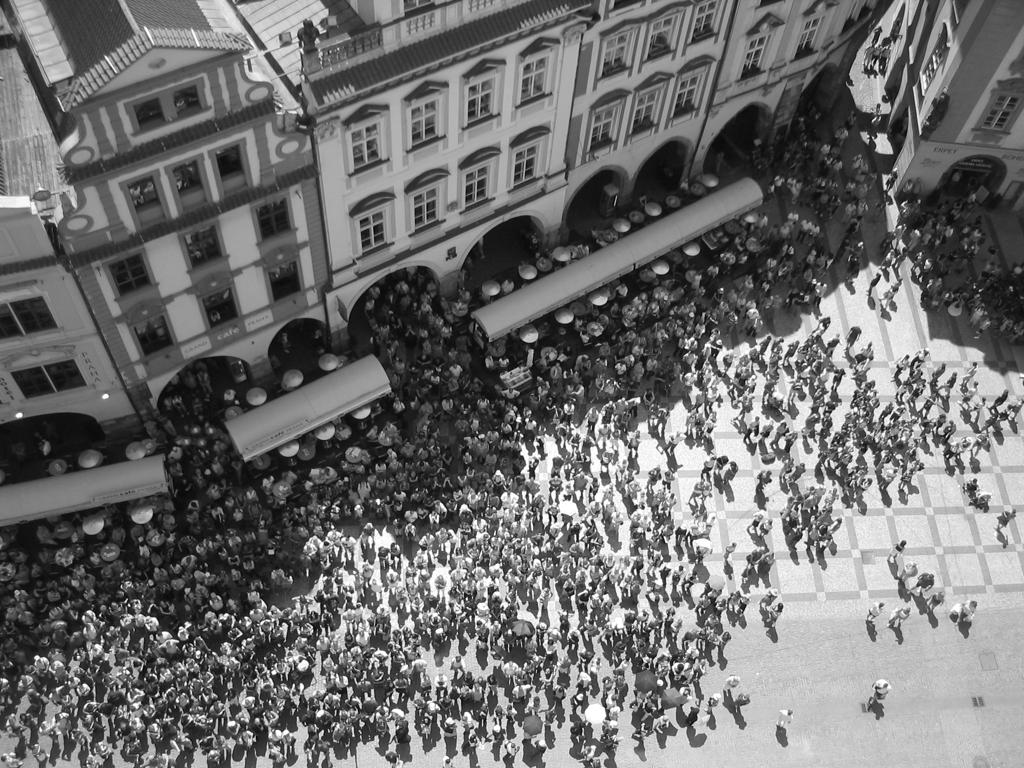
\includegraphics[width=\textwidth]{crowd}
			\caption{Crowd}
		\end{figure}
	\end{column}
	\begin{column}{.5\textwidth}
		\begin{figure}[ht]
			\centering
			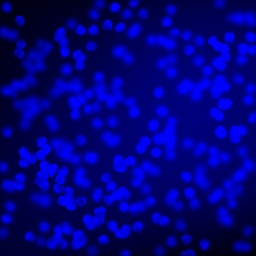
\includegraphics[width=\textwidth]{cells}
			\caption{Cells}
		\end{figure}
	\end{column}
\end{columns}
\end{frame}

\begin{frame}{Datasets}
\begin{columns}
	\begin{column}{.5\textwidth}
		\begin{figure}[ht]
			\centering
			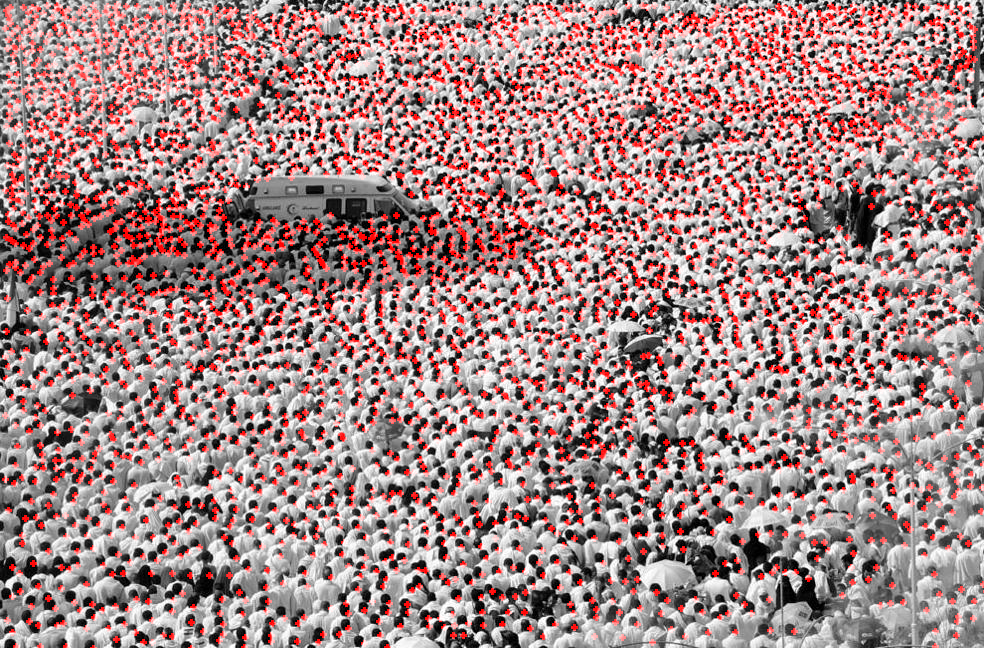
\includegraphics[width=\textwidth]{annotation}
			\caption{Crowd Annotation}
		\end{figure}
	\end{column}
	\begin{column}{.5\textwidth}
		\begin{itemize}
			\item Annotated images
			\begin{itemize}
				\item 50 crowd , 200 cell picture
				\item Local information
			\end{itemize}
		\end{itemize}
	\end{column}
\end{columns}
\end{frame}

\section{Architecture}

%\begin{frame}{Patch based counting}
%\begin{figure}[ht]
%	\centering
%	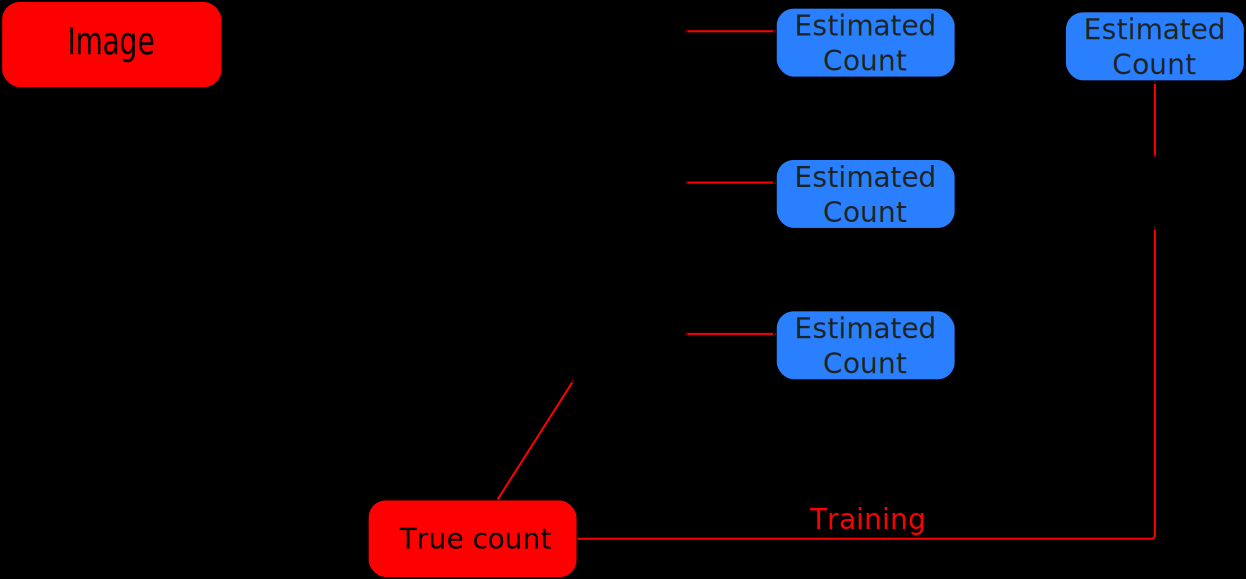
\includegraphics[width=\textwidth]{architecture_training}
%	\caption{Training}
%\end{figure}
%\end{frame}
%
%\begin{frame}{Patch based counting}
%\begin{figure}[ht]
%	\centering
%	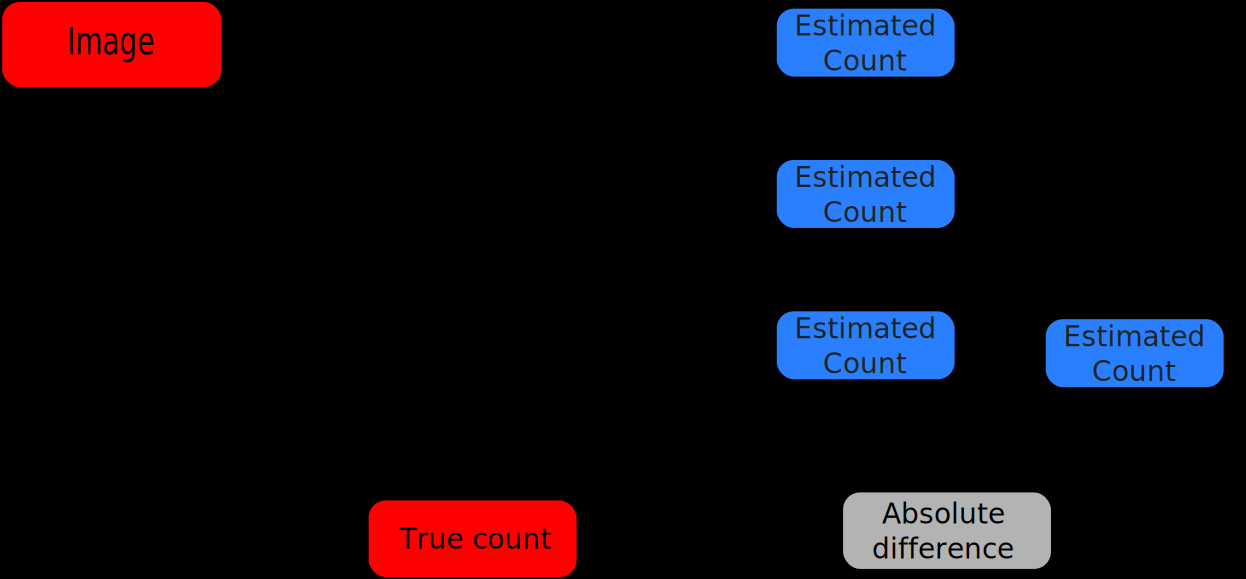
\includegraphics[width=\textwidth]{architecture_test}
%	\caption{Testing}
%\end{figure}
%\end{frame}

\subsection{Overview}

\begin{frame}{Comparative work}
\begin{tabular}{p{.30\textwidth}|p{.30\textwidth}|p{.30\textwidth}}
\hline
\textbf{Data} & \textbf{Features} & \textbf{Counting Alg.}\\
\hline
Cells & Dense SIFT & Pixel based \\
&& \\
Crowd & Fourier, sparse SIFT, head detection & Patch based\\
&& \\
& CNN layers &\\
\end{tabular}
\end{frame}

\subsection{Regressors}

% Define block styles
\tikzstyle{decision} = [rectangle, draw, fill=green!20, text centered, rounded corners, minimum height=2em,text width=3em]
\tikzstyle{block} = [rectangle, draw, fill=blue!20,  text centered, rounded corners, minimum height=2em,text width=3em]
\tikzstyle{line} = [draw, -latex']
\tikzstyle{redline} = [draw, color=red, -latex']
\tikzstyle{result} = [rectangle, draw, fill=red!20, text centered, rounded corners, minimum height=2em,text width=3em]
\tikzstyle{count} = [rectangle, draw, fill=yellow!20, text centered, rounded corners, minimum height=2em,text width=3em]

\begin{frame}{Pixel based counting}
	\begin{tikzpicture}[auto,node distance=1.8cm and 7cm,>=latex]
		\node [result] (image) {Image};
		\node [count, right = 2cm of image] (density) {Density $F^0$};
		\node [block, below of=image] (feature) {Feature field $\mathbf{d}$};
		\node [count, right = 2cm of feature, text width = 5em] (estimated) {Estimated density $F$};
		\node[decision, above right = -0.2cm and 1cm of estimated, text width=4em] (mesa) {MESA distance};
		\path[line] (image) -- (density);
		\path[line] (feature) to node[midway] (t) {$\textbf{w}^Tb$} (estimated);
		\path[line]  (density) -- (mesa);
		\path[line] (estimated) -- (mesa);
		\onslide<1-2>{
		\node[below = 2cm of mesa] (mesa_for) {\small
		$D_{MESA}(F,F^0)=\,\max_{B \in \mathbf(B)} \vert \sum_{p \in B}F(p)-\sum_{p \in B}F^0(p) \vert$
		};
		\path[line] (mesa) -- (mesa_for);
		}
		\onslide<2>{
		\path[redline] (mesa.south) to [out=-90,in=-90] node[above, color=red] {Training} (t.south);
		}
		\onslide<3>{
		\node[result,right = 1cm of mesa] (ad) {AD};
	   	\path[line,color=blue] (density.east) to [out=0,in=135] node[above, color=blue] {Test} (ad.north);
	   	\path[line,color=blue] (estimated.east) to [out=0,in=-135] (ad.south);
	   	}
	\end{tikzpicture}
\end{frame}


\begin{frame}{Patch based counting}	    
	\begin{tikzpicture}[auto,node distance=1.8cm and 7cm,>=latex]
	    % Place nodes
	    \node [result] (image) {Image};
	    \node [result,right of=image] (patch1) {Patch};
	    \node [result,above of=patch1] (patch2) {Patch};
	    \node[count,below of=patch1] (truecount) {True count};  
	    \node [right of=patch2] (a) {};
	    \path [line] (image) -- (patch1);
	    \path [line] (image) -- (patch2);
		\path [line] (patch1) -- (truecount);	 
		\path [line,dashed] (patch2) -- (a);	
		   
	    \node [block,right of=patch1] (features1) {Head detection};
	   	\node [decision, right of=features1] (SVM1) {SVM};
	   	\node [count, right of=SVM1] (estimated1) {Count};
	   	\path [line] (patch1) -- (features1);
	   	\path [line] (features1) -- (SVM1);
	   	\path [line] (SVM1) -- (estimated1)
	   	;
		\node [block,below of=features1](features2) {Fourier};
	   	\node [decision, right of=features2] (SVM2) {SVM};
	   	\node [count, right of=SVM2] (estimated2) {Count};
	   	\path [line] (patch1) -- (features2);
	   	\path [line] (features2) -- (SVM2);
	   	\path [line] (SVM2) -- (estimated2);	   	
	   	
	   	\node [block,below of=features2](features3) {Sparse SIFT};
	   	\node [decision, right of=features3] (SVM3) {SVM};
	   	\node [count, right of=SVM3] (estimated3) {Count};
	   	\path [line] (patch1) -- (features3);
	   	\path [line] (features3) -- (SVM3);
	   	\path [line] (SVM3) -- (estimated3);
	  
	  	\node[decision,right of=estimated2] (SVM) {SVM};
	  	\node[count, below of=SVM] (estimated) {Count};
	  	\path [line] (estimated1) -- (SVM);
	  	\path [line] (estimated2) -- (SVM);
	  	\path [line] (estimated3) -- (SVM);
	   	\path[line] (SVM) -- (estimated);
	   	
	   	\onslide<2>{
	   	\path[redline] (truecount) -- (SVM1);
	   	\path[redline] (truecount) -- (SVM2);
	   	\path[redline] (truecount) -- (SVM3) ;
	   	\path[redline] (truecount.north) to [out=90,in=90] node[above, color=red] {Training} (SVM.north);
	   	}
	   	
	   	\onslide<3>{
	   	\node[result,below of=truecount] (ad) {AD};
	   	\path[line,color=blue] (truecount) -- (ad);
	   	\path[line,color=blue] (estimated.south) to [out=-135,in=-45] node[above, color=blue] {Test} (ad.south);
	   	}
	    % Draw edges
%	    \path [line] (decide) -| node [near start] {yes} (update);
%	    \path [line] (update) |- (identify);
%	    \path [line] (decide) -- node {no}(stop);
%	    \path [line,dashed] (expert) -- (init);
%	    \path [line,dashed] (system) -- (init);
%	    \path [line,dashed] (system) |- (evaluate);
	\end{tikzpicture}
\end{frame}

\begin{frame}{MRF regularisation}
$$E(l) = \sum_{p \in \mathcal{V}}D_p(l_p) + \sum_{(p,q)\in \mathcal{N}}V(l_p-l_q))$$
\begin{columns}[t]
	\begin{column}{.33\textwidth}
		\begin{figure}[ht]
			\centering
			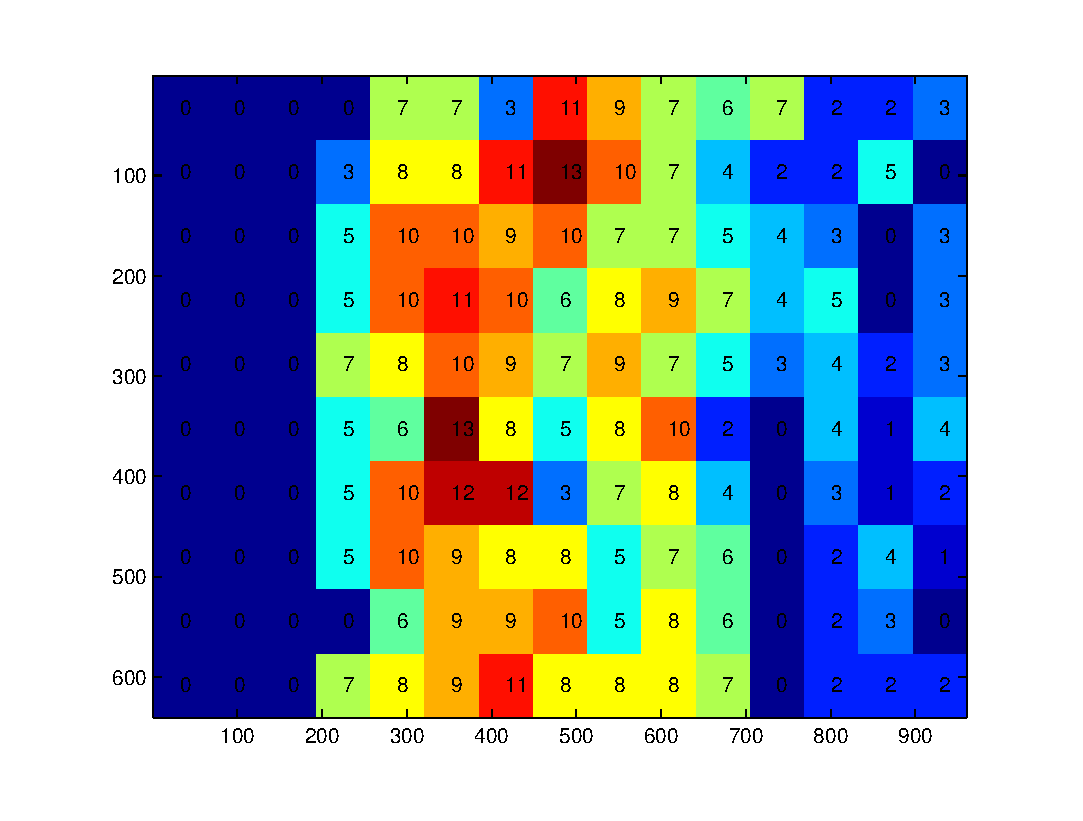
\includegraphics[width=\textwidth]{mrf_true.eps}
			\caption{True density}
		\end{figure}
	\end{column}
	\begin{column}{.33\textwidth}
		\begin{figure}[ht]
			\centering
			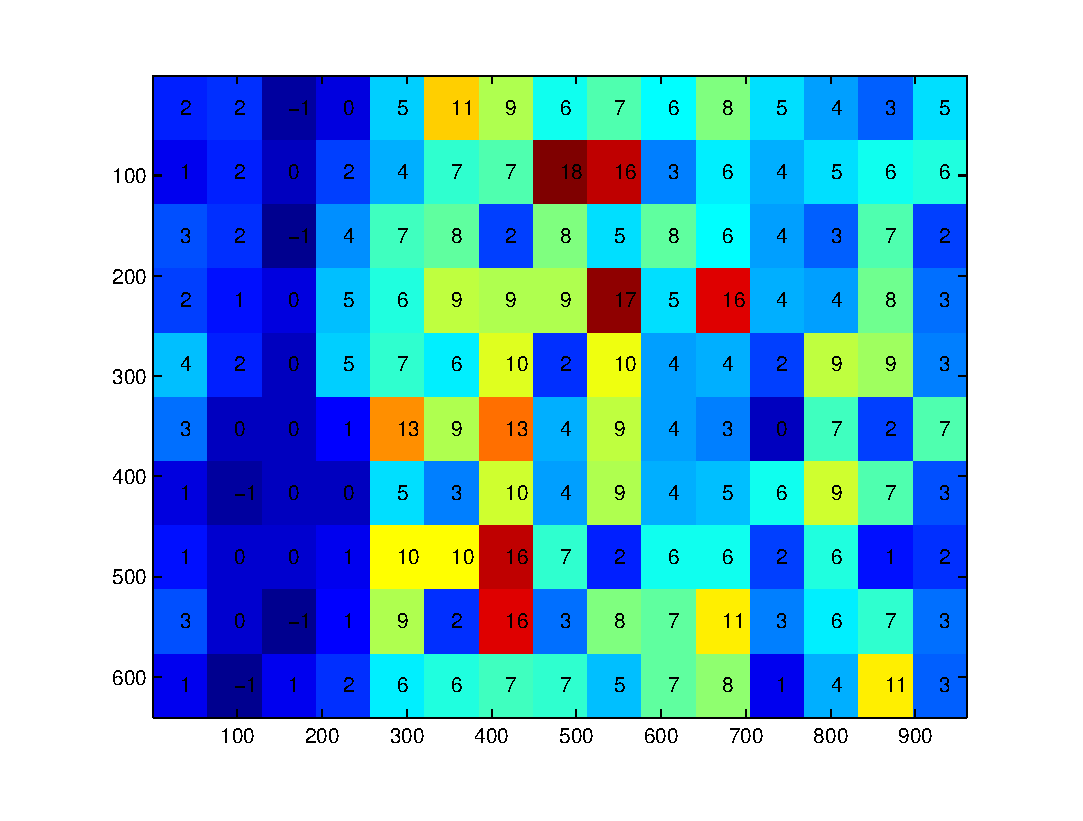
\includegraphics[width=\textwidth]{mrf_before.eps}
			\caption{Before MRF}
		\end{figure}
	\end{column}
	\begin{column}{.33\textwidth}
		\begin{figure}[ht]
			\centering
			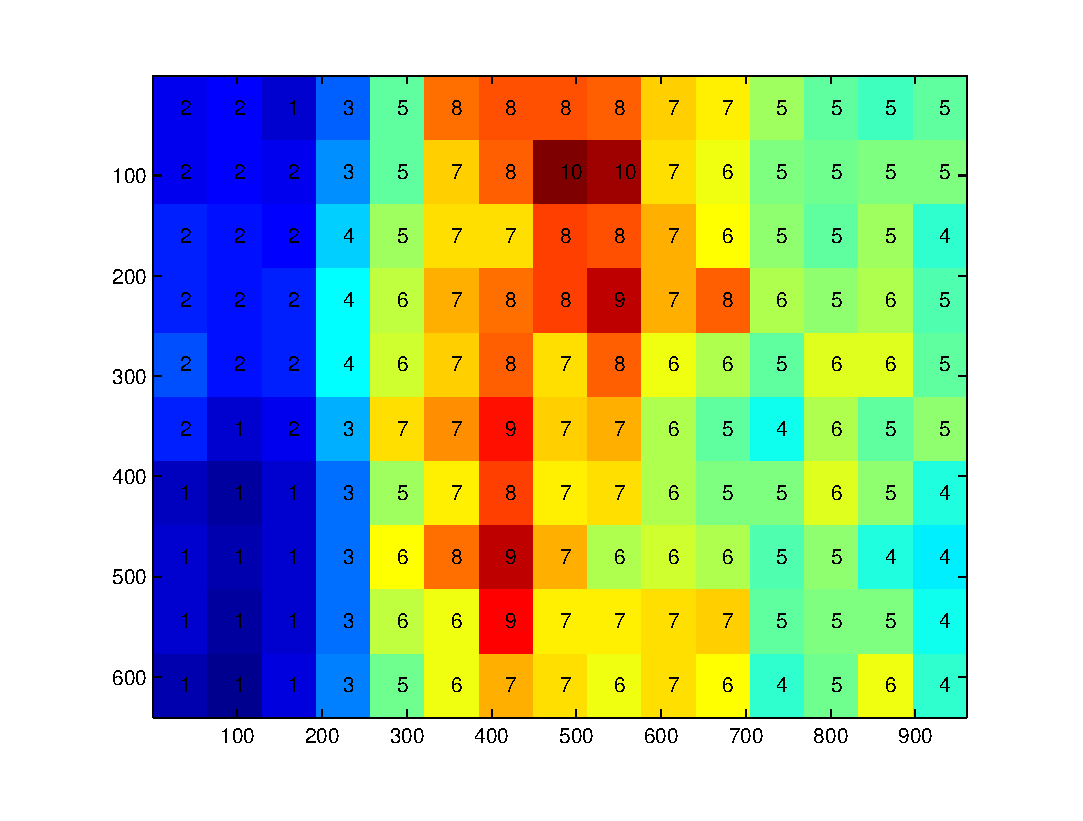
\includegraphics[width=\textwidth]{mrf_after.eps}
			\caption{After MRF}
		\end{figure}
	\end{column}
\end{columns}
\end{frame}
\subsection{Features}

%\begin{frame}{Dense SIFT}
%\begin{columns}
%	\begin{column}{.5\textwidth}
%		\begin{figure}[ht]
%			\centering
%			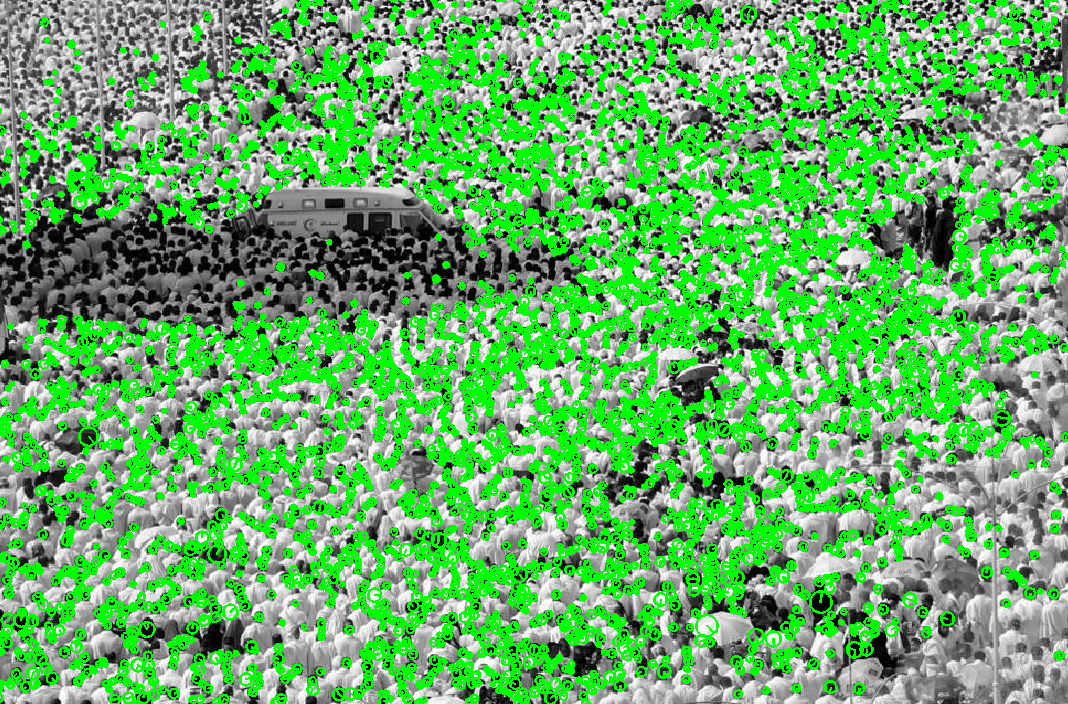
\includegraphics[width=\textwidth]{sift}
%			\caption{Dense SIFT}
%		\end{figure}
%	\end{column}
%	\begin{column}{.5\textwidth}
%		\begin{itemize}
%			\item Dense
%			\item Vocabulary based feature
%			\begin{itemize}
%				\item Nearest neighbor cluster
%			\end{itemize}
%		\end{itemize}
%	\end{column}
%\end{columns}
%\end{frame}

\begin{frame}{Combining patch features}
\begin{columns}[t]
	\begin{column}{.33\textwidth}
		\begin{figure}[ht]
			\centering
			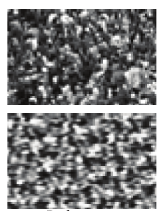
\includegraphics[width=\textwidth]{fourier}
			\caption{Fourier filtered maximum detection}
		\end{figure}
	\end{column}
	\begin{column}{.33\textwidth}
		\begin{figure}[ht]
			\centering
			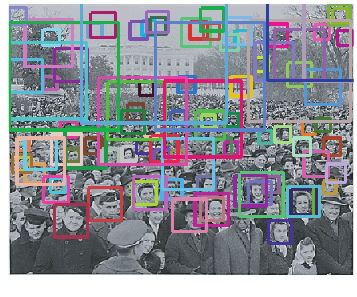
\includegraphics[width=\textwidth]{head_detection}
			\caption{Deformable model based head detection}
		\end{figure}
		\begin{itemize}
			\item Confidence
		\end{itemize}
	\end{column}
	\begin{column}{.33\textwidth}
		\begin{figure}[ht]
			\centering
			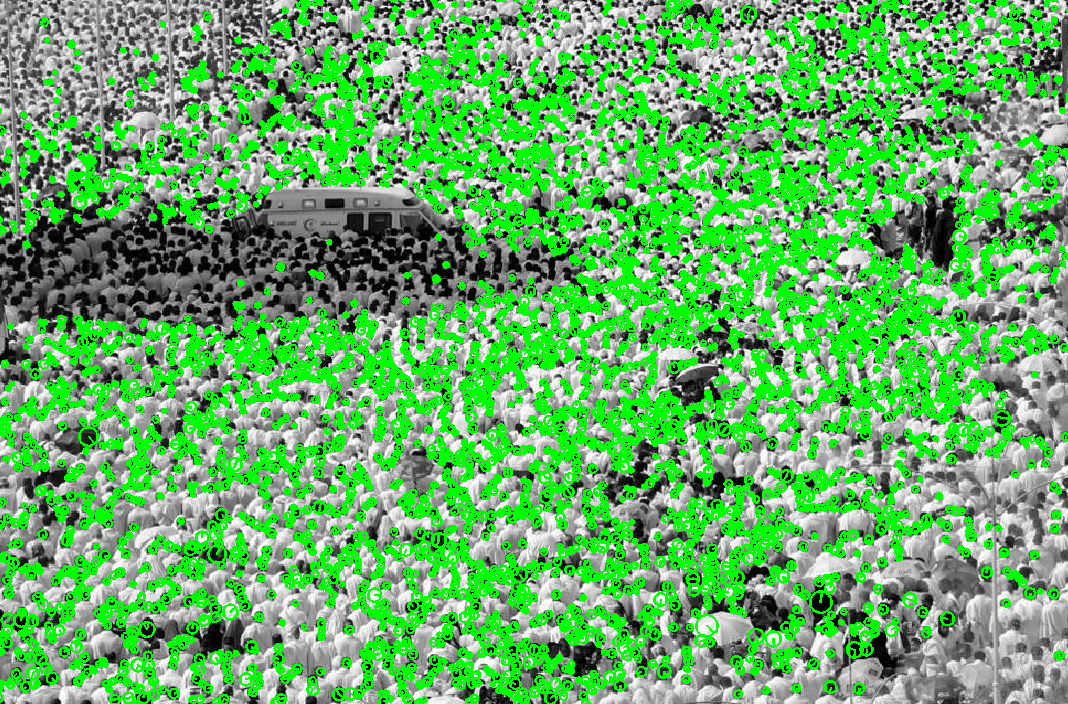
\includegraphics[width=\textwidth]{sift}
			\caption{Sparse SIFT}
		\end{figure}
		\begin{itemize}
			\item Histogram features
			\item Confidence
		\end{itemize}
	\end{column}
\end{columns}
\end{frame}

\begin{frame}{Overfeat}
    \begin{itemize}
    \item remove all pooling layers
    \item remove all stride parameters for convolutional layers
  \end{itemize}
  \begin{table}
  \tiny
    \begin{tabular}{|c|c|c|c|c|c|c|c|} \hline
    version & 1 & 2 & 3 & 4 & 5 & 6 & filter size \\ \hline
    layers & conv1 & conv1 & conv1 & conv1 & conv1 & conv1 & $ 11 \times 11 \times 64$ \\ 
    & ReLU & ReLU & ReLU & ReLU & ReLU & ReLU & \\
    & Norm & Norm & Norm & Norm & Norm & Norm & \\
    & conv2 & conv2 & conv2 & conv2 & conv2 & conv2&  $ 5 \times 5 \times 256$ \\
    &  & ReLU & ReLU & ReLU & ReLU & ReLU & \\
    &  & Norm & Norm & Norm & Norm & Norm & \\
    & & & conv3 & conv3 & conv3 & conv3 &  $3 \times 3 \times 256 $\\
    &  &  & ReLU & ReLU & ReLU & ReLU & \\
    &  &  &  & conv4 & conv4 & conv4 &  $3 \times 3 \times 256 $\\
    &  &  &  & ReLU & ReLU & ReLU & \\
    &  &  &  &  & conv5 & conv5 &  $3 \times 3 \times 256 $\\
    &  &  &  &  & ReLU & ReLU & \\
    &   &   &   &  &  & conv6 &  $6 \times 6 \times 4096 $\\
    &  &  &  &  &  & ReLU & \\ \hline
    \end{tabular}
  \end{table}
\end{frame}

\section{Results}

\subsection{Validation}
\begin{frame}{Validation method}
  \begin{itemize}
  \item Limited dataset
  \item K-fold technics:
	  \begin{itemize}
	    \item Training on $20\%$ of the set
	    \item Validating hyper-parameters on $20\%$ of the set
	    \item Testing on $60\%$ of the set
	  \end{itemize}
  \item Set split at random
	    \begin{itemize}
	    \item Repeated 5 times to average results
	    \item Mean + variance
	  \end{itemize}
  \end{itemize}
\end{frame}

\subsection{Cells}
\begin{frame}{Cells}
\begin{itemize}
\item Original results (from paper)
\begin{table}
\tiny
\begin{tabular}{|c|c|c|c|c|c|c|}
\hline
Validation & $N=1$ & $N=2$ & $N=4$ & $N=8$ & $N=16$ & $N=32$ \\ \hline
counting & $12.7 \pm 7.3$ & $7.8 \pm 3.7$ & $5.0 \pm 0.5$ & $4.6 \pm 0.6$ & $4.2 \pm 0.4$ & $3.6 \pm 0.2$ \\ \hline
MESA & $9.5 \pm 6.1$ & $6.3 \pm 1.2$ & $4.9 \pm 0.6$ & $4.9 \pm 0.7$ & $3.8 \pm 0.2$ & $3.5 \pm 0.2$ \\ \hline
\end{tabular}
\normalsize
\end{table}

\item Reproduced SIFT results
\begin{table}
\tiny
\begin{tabular}{|c|c|c|c|c|c|c|}
\hline
Validation & $N=1$ & $N=2$ & $N=4$ & $N=8$ & $N=16$ & $N=32$ \\ \hline
counting & $28.6 \pm 11.6$ & $16.4 \pm 4.4$ & $8.5 \pm 1.1$ & $7.2 \pm 0.9$ & $6.5 \pm 0.5$ & $5.5 \pm 0.5$ \\ \hline
MESA & $26.1 \pm 5.2$ & $13.5 \pm 2.7$ & $8.9 \pm 1.4$ & $6.7 \pm 0.5$ & $6.9 \pm 0.3$ & $5.5 \pm 0.3$ \\ \hline
\end{tabular}
\normalsize
\end{table}

\item Overfeat results
\begin{table}
\tiny
\begin{tabular}{|c|c|c|c|c|c|}
\hline
& NET 1 & NET 2 & NET 3 & NET 4 & NET 5 \\
nFeatures & $N=16$ & $N=16$ & $N=16$ & $N=16$ & $N=16$  \\ \hline
256 & $3.7 \pm 0.3$ & $3.8 \pm 0.4$ & $3.7 \pm 0.1$ & $3.9 \pm 0.2$ & $3.8 \pm 0.4$ \\ \hline
512 & $3.4 \pm 0.2$ & $3.5 \pm 0.3$ & $3.7 \pm 0.2$ & $3.5 \pm 0.3$ & $3.6 \pm 0.2$ \\ \hline
\end{tabular}
\normalsize
\end{table}
\end{itemize}
\end{frame}
\subsection{Crowd}

\begin{frame}{Crowd - CNN}

Error can be hard to estimate because of high variance. Best result obtained: $484.0 \pm 528.3$.

\begin{table}
\tiny

\begin{tabular}{@{}|c|c|c|c|c|c|c|@{}}
\hline
Nfeatures & $CNN 1$ & $CNN 2$ & $CNN 3$ & $CNN 4$ & $CNN 5$ & $CNN 6$ \\ \hline
512 & $615 \pm 591$ & $636 \pm 597$ & $657 \pm 589$ & $638 \pm 579$ & $628 \pm 596$ & $484 \pm 528$ \\ \hline
1024 & $614 \pm 607$ & $ 602 \pm 589$ & $567 \pm 567$ & $530 \pm 540$ & $547 \pm 589$ & $574 \pm 583$ \\ \hline
\end{tabular}
\normalsize
\end{table}

\end{frame}

\begin{frame}{Crowd - All algorithms}
\begin{figure}
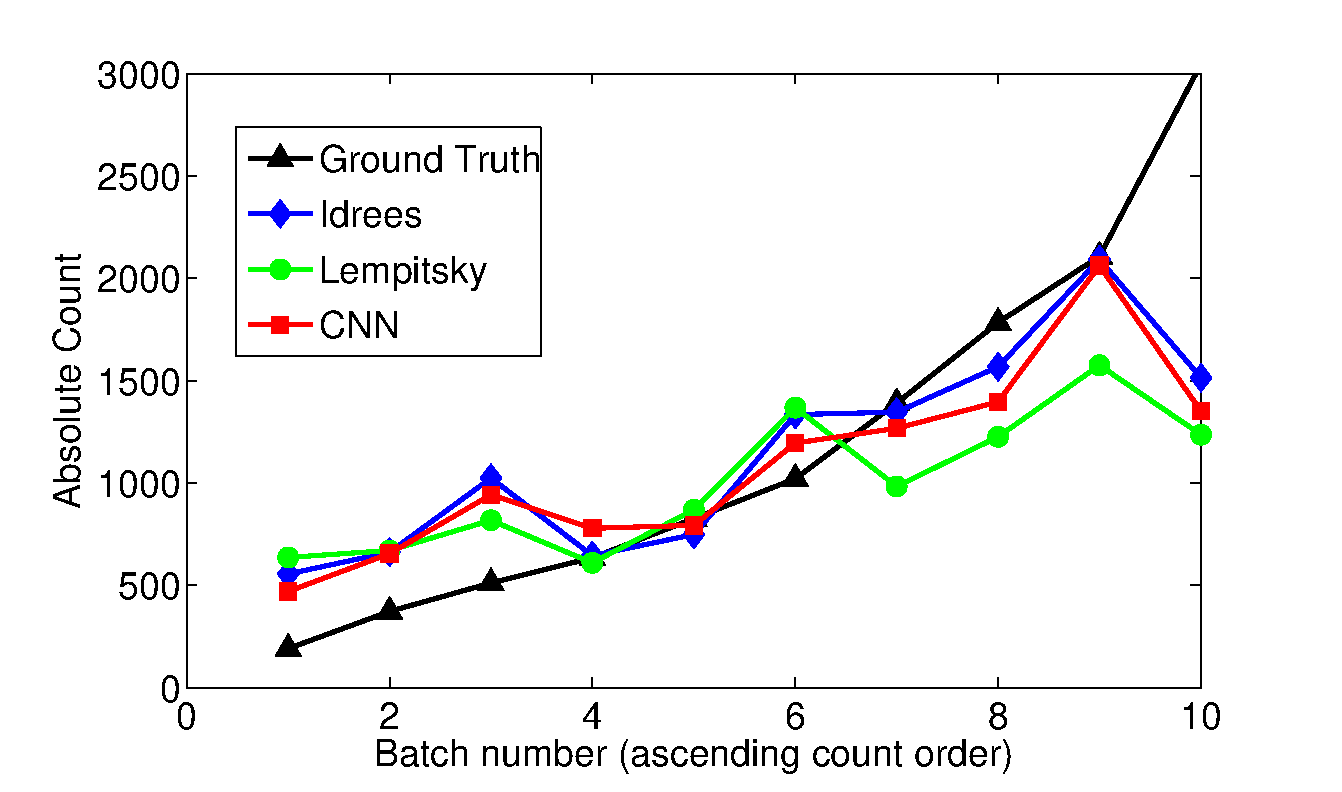
\includegraphics[width=\textwidth]{good_compare.eps}
\end{figure}
\end{frame}


\begin{frame}{Crowd - All algorithms}
\begin{figure}
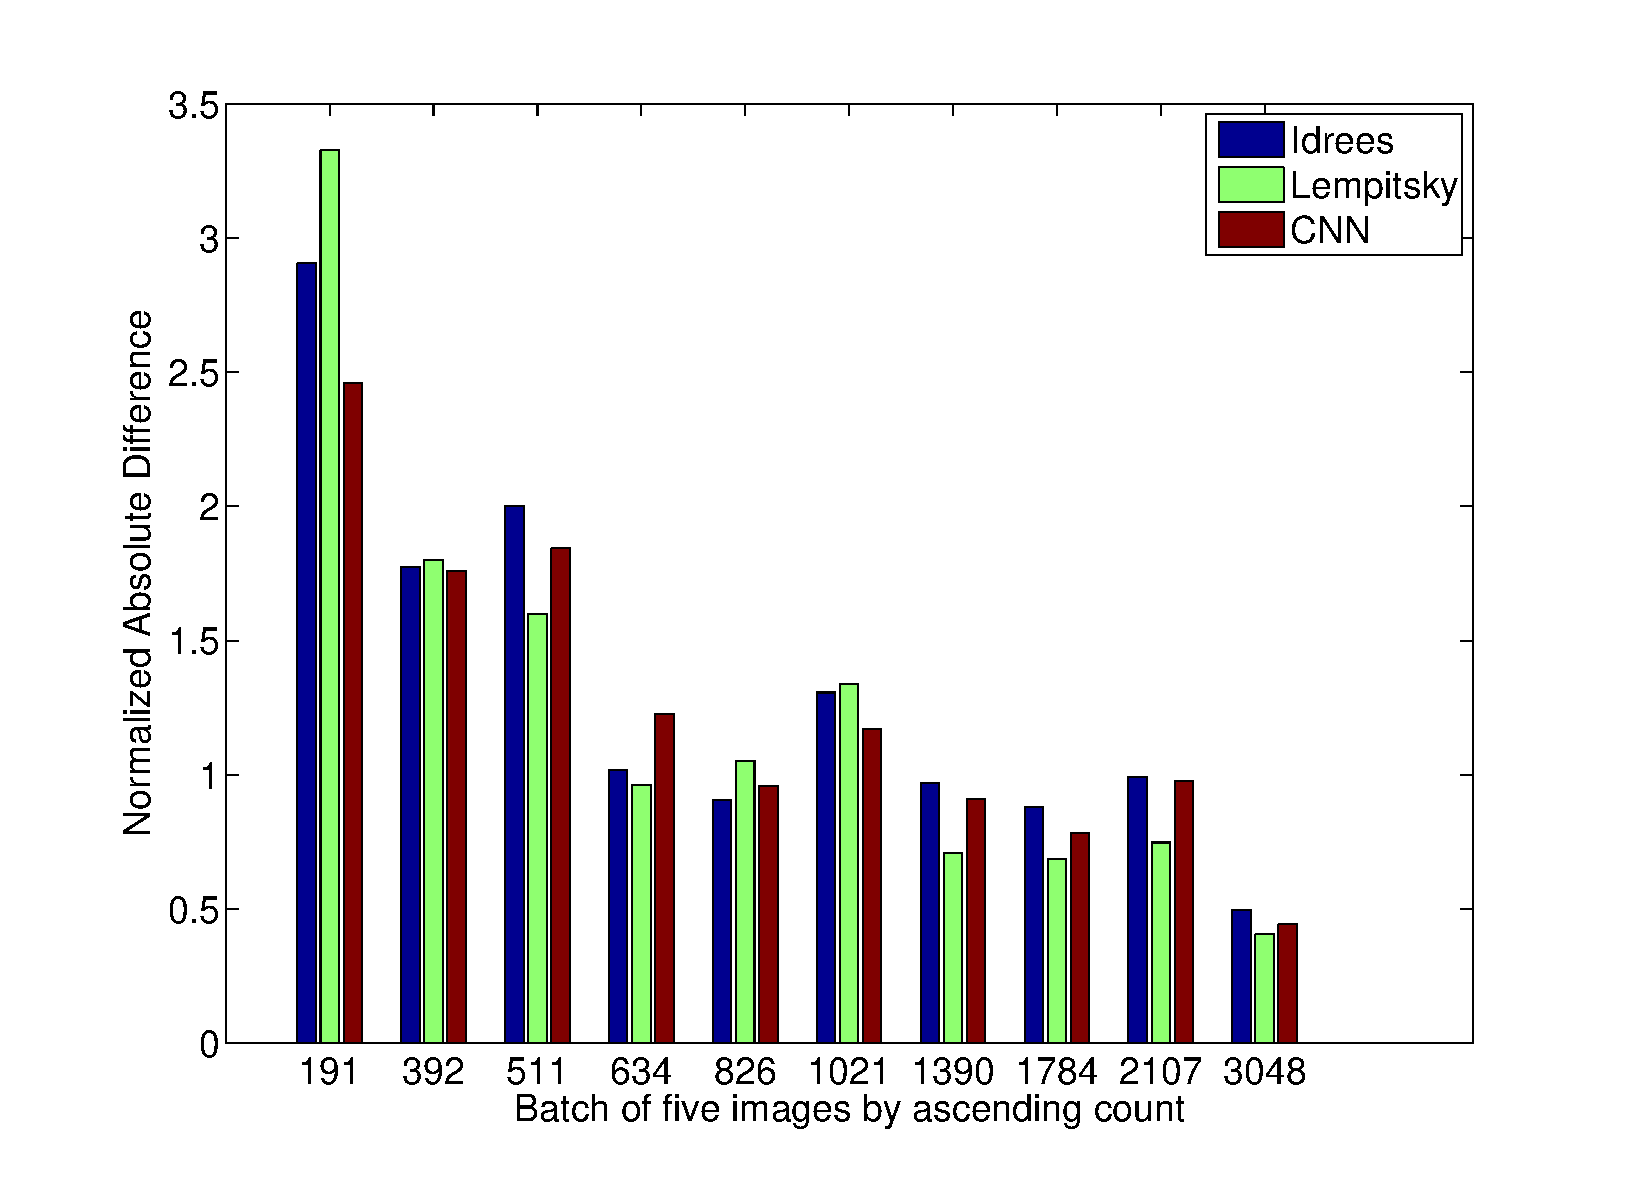
\includegraphics[width=\textwidth]{good_compare_bar.eps}
\end{figure}
\end{frame}

\section*{Conclusion}
\begin{frame}{Conclusion}
Results of different methods on the {\bf crowd} dataset :
\begin{figure}
 \centering
  \begin{tabular}{|c|c|}

\hline
Dense SIFT & $466 \pm 481$  \\ \hline
Combined Features & $523 \pm 603$  \\ \hline
CNN & $464 \pm 516$  \\ \hline
\end{tabular}
 \end{figure}


\vspace{0.25cm}
\begin{itemize}
 \item MRF Regularization didn't yield any noticeable improvement on those results yet.

 \item Are these results significant ?
\end{itemize}


\end{frame}
\end{document}
